\documentclass{standalone}
\usepackage{pgfplots}
\pgfplotsset{compat=newest}

\begin{document}
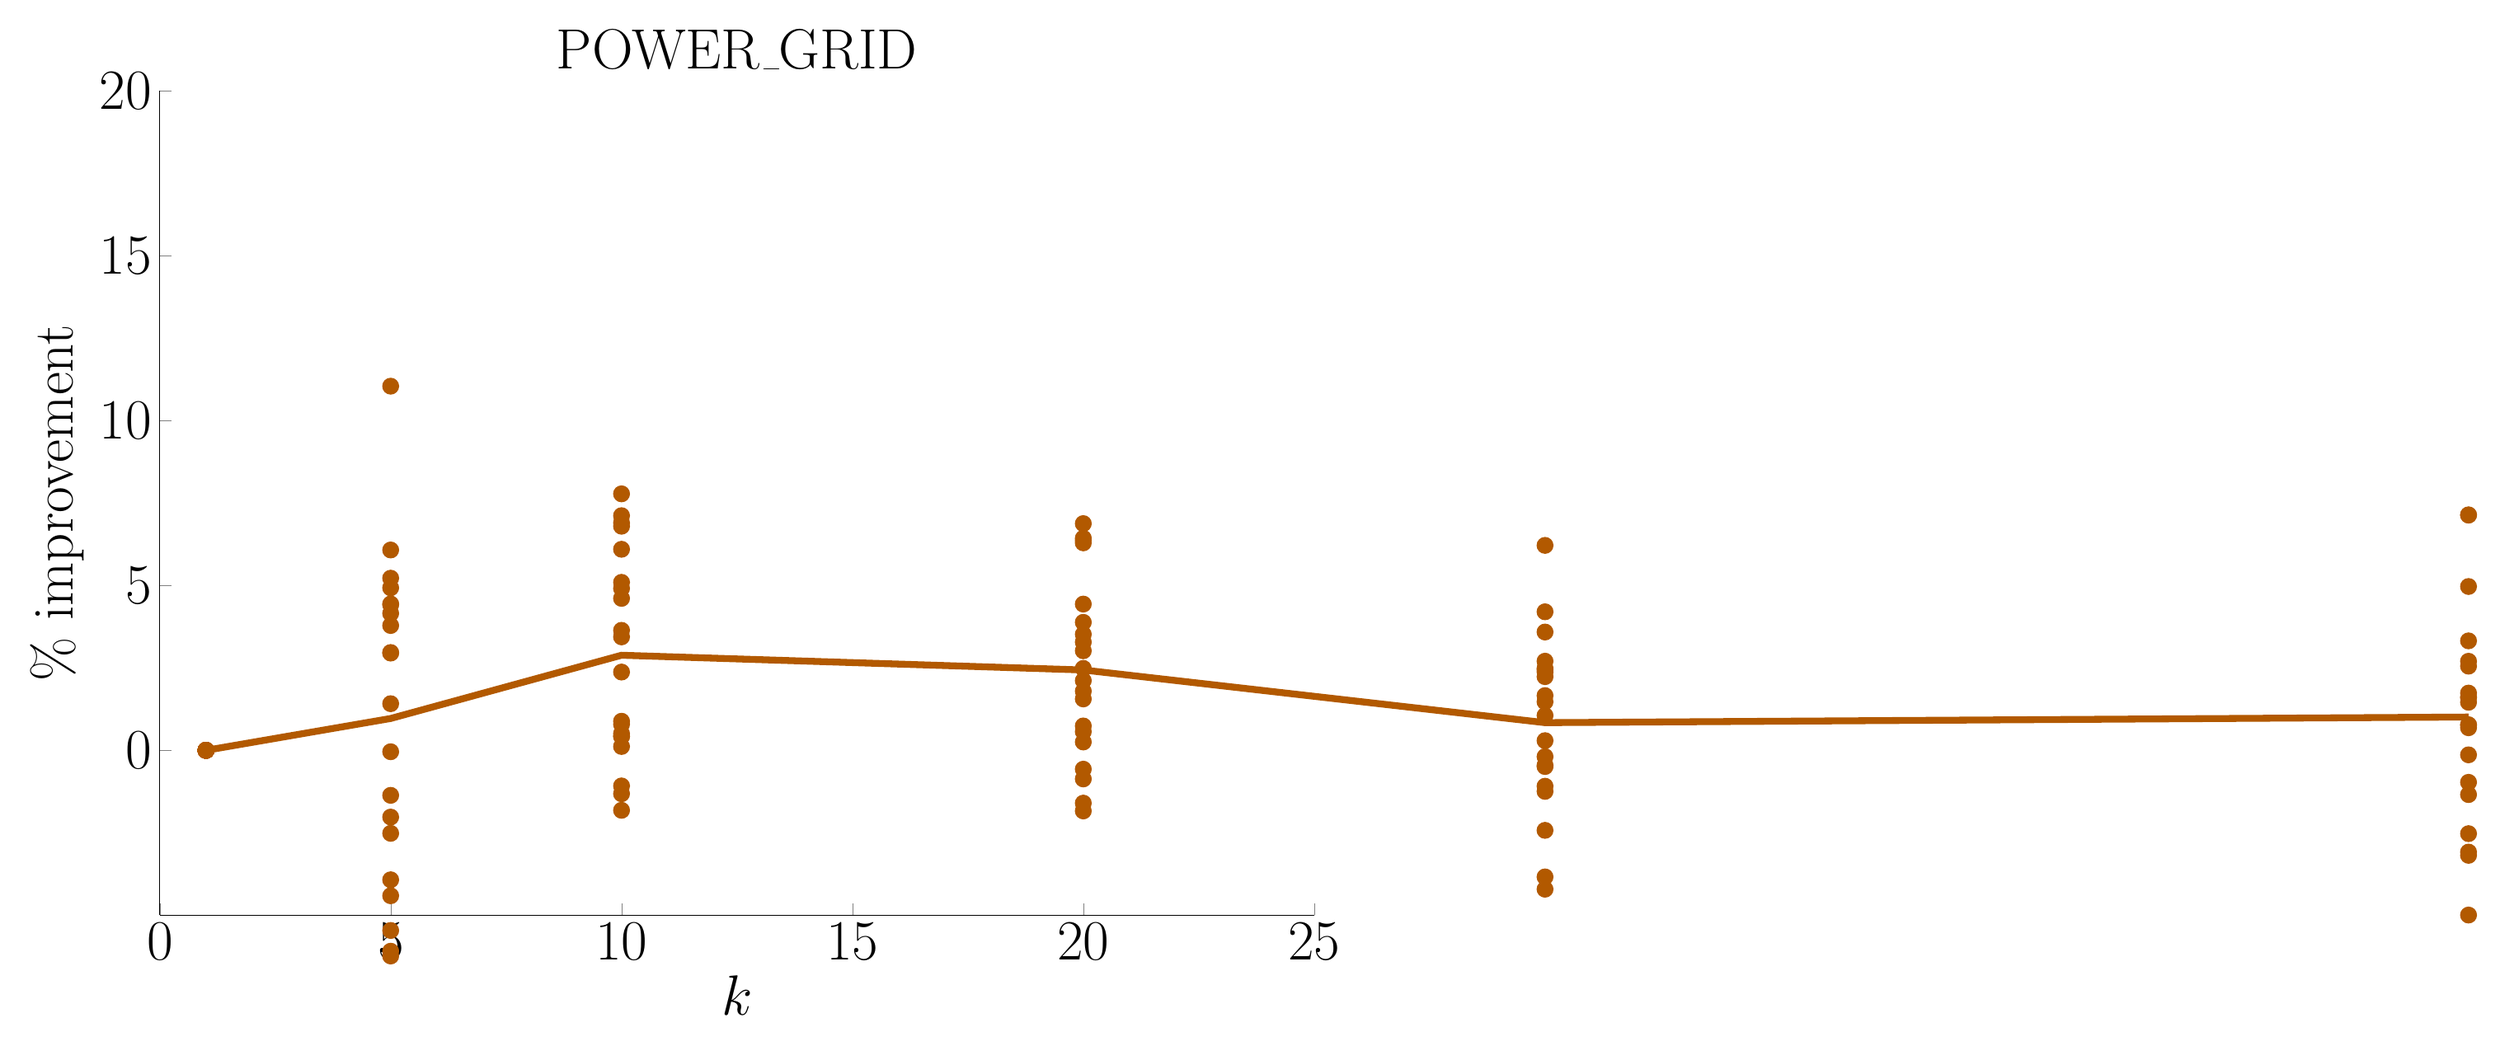
\begin{tikzpicture}

\begin{axis}[%
title style={font=\Huge},
title=POWER\_GRID,
tick label style={font=\Huge},
label style={font=\Huge},
legend style={font=\Huge},
view={0}{90},
width=7in,
height=5in,
scale only axis,
xmin=0, xmax=25,
xtick={0, 5, 10, 15, 20, 25},
xlabel={$k$},
ymin=-5, ymax=20,
ytick={0, 5, 10, 15, 20},
ylabel={$\%$ improvement},
major tick length=5pt,
axis lines*=left,
legend cell align=left,
clip=false]

\addplot [
only marks,
mark=*,
mark size=3.5pt,
color=orange!70!black,
%solid,
%line width=2pt,
]
coordinates{
(1,0.0)(1,0.0)(1,0.0)(1,0.0)(1,0.0)(1,0.0)(1,0.0)(1,0.0)(1,0.0)(1,0.0)(1,0.0)(1,0.0)(1,0.0)(1,0.0)(1,0.0)(1,0.0)(1,0.0)(1,0.0)(1,0.0)(1,0.0)(5,-6.23781676413)(5,-6.09202851588)(5,-5.46341463415)(5,-4.41014332966)(5,-3.92584514722)(5,-2.51762336354)(5,-2.02385254789)(5,-1.36518771331)(5,-0.0424989375266)(5,1.41458106638)(5,2.94985250737)(5,2.96735905045)(5,3.78594830724)(5,4.15276232851)(5,4.4173327724)(5,4.44007858546)(5,4.92957746479)(5,5.2217453505)(5,6.07692307692)(5,11.0451306413)(10,-1.81854121368)(10,-1.31628431741)(10,-1.07913669065)(10,0.117073170732)(10,0.419748151109)(10,0.43233895374)(10,0.506822612086)(10,0.789754535752)(10,0.882594417077)(10,2.37439050244)(10,3.44095157179)(10,3.63959165557)(10,4.60876689881)(10,4.91191709845)(10,5.09580105993)(10,6.09806345282)(10,6.79728108756)(10,6.90010298661)(10,7.11690532165)(10,7.77957860616)(20,-1.83840749415)(20,-1.60063571347)(20,-0.867365377665)(20,-0.571095571096)(20,0.252941823381)(20,0.566315551025)(20,0.739713361073)(20,1.55910079768)(20,1.79477658126)(20,2.11495396865)(20,2.48518011856)(20,3.01938369781)(20,3.28282828283)(20,3.51888901965)(20,3.88216487783)(20,4.43567670971)(20,6.2924959822)(20,6.36795324486)(20,6.4336372847)(20,6.87732342007)(30,-4.21168129642)(30,-3.8392011707)(30,-2.42681374629)(30,-1.24474203794)(30,-1.08815778288)(30,-0.491209927611)(30,-0.453857791225)(30,-0.191021967526)(30,0.294117647059)(30,1.05633802817)(30,1.47304988283)(30,1.66008614501)(30,2.23503325942)(30,2.37422771403)(30,2.44817726948)(30,2.48685637987)(30,2.70411268585)(30,3.58841692398)(30,4.20198055134)(30,6.21619143669)(50,-4.99542752629)(50,-3.18463880108)(50,-3.08590984187)(50,-2.52682369373)(50,-1.34224219489)(50,-0.96950467125)(50,-0.136747886624)(50,0.684693048625)(50,0.76651660786)(50,0.776204669647)(50,1.45777997406)(50,1.59466327827)(50,1.61877274438)(50,1.73659525922)(50,2.5533445217)(50,2.70189312245)(50,3.32061324228)(50,4.96926560983)(50,7.13360952874)(50,7.14285714286)
};

\addplot [
color=orange!70!black,
solid,
line width=3pt
]
coordinates{
(1,0.0)(5,0.966144009903)(10,2.88488599303)(20,2.43729152825)(30,0.839595110157)(50,1.01077570671)
};

\end{axis}
\end{tikzpicture}
\end{document}
